\documentclass[11pt]{article}
%Importing custom commands
\usepackage{latex_goon/latex_goon}
\title{Decoder-Only Transformers}
\author{Garrett Goon}
\begin{document}
%
%\maketitle

\vspace{1truecm}
%
%
\renewcommand{\thefootnote}{\fnsymbol{footnote}}
\begin{center}
{\huge \bf{Decoder-Only Transformers}}
\end{center}


\begin{abstract}

Notes on various aspects of Decoder-Only Transformers.

\end{abstract}

\tableofcontents


\renewcommand*{\thefootnote}{\arabic{footnote}}
\setcounter{footnote}{0}

\part{Architecture}

\section{Decoder-Only Fundamentals \label{sec_decoder_only} }

The Transformers architecture \cite {vaswani2017attention}, which dominates Natural Language
Processing (NLP) as of July 2023, is a relatively simple architecture. There are various flavors and
variants of Tranformers, but focus here on the decoder-only versions which underlie the
GPT models \cite {gpt2radford2019language, gpt3brown2020language, gpt4openai2023}.

The full decoder-only architecture can be seen in Fig.~\ref{fig:transformers_architecture}. The
parameters which define the network can be found in App.~\ref{app_conventions}.
\begin{figure}[ht]
    \centering
    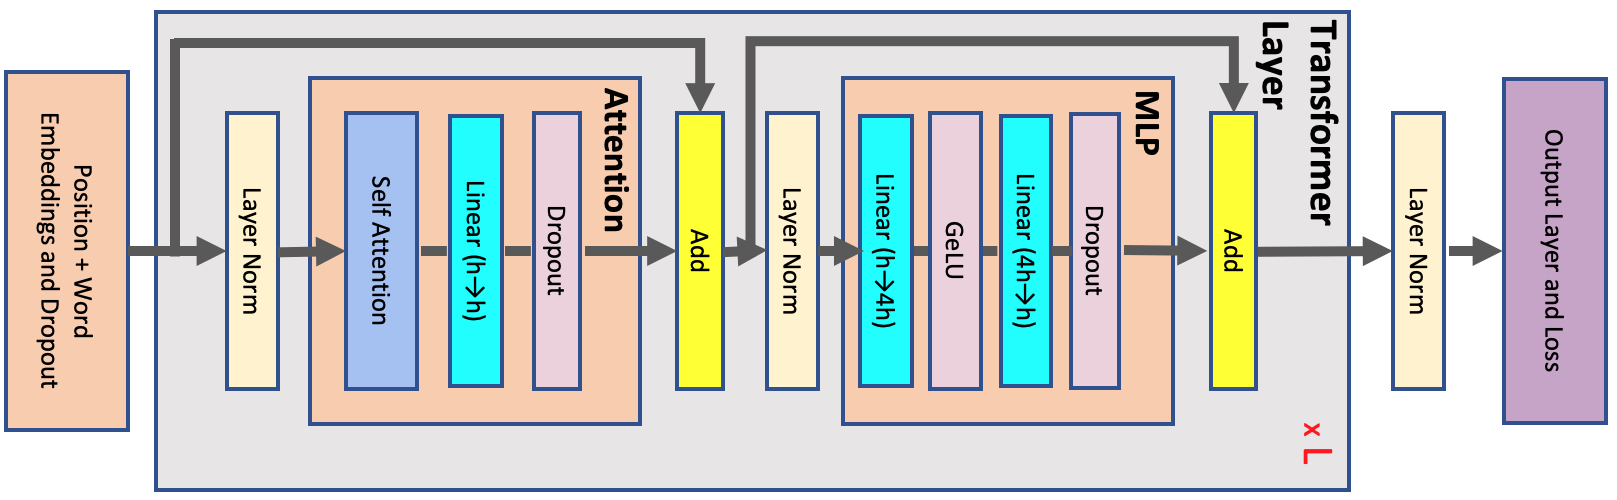
\includegraphics[scale=0.28]{figures/transformer-general.jpg}
    \caption{The full transformers architecture. Diagram taken from \cite{korthikanti2022reducing} }
    \label{fig:transformers_architecture}
\end{figure}


An outline of the mechanics:
\begin{enumerate}
    \item Raw text is \textbf{tokenized} and turned into a series of integers\footnote{There are
        about \href{https://github.com/ray-project/llm-numbers}{1.3 tokens per word}, on average.} whose values lie in \pyinline{range(V)}, with $ V $ the vocabulary
        size.
    \item The tokenized text is chunked and turned into \pyinline{(B, S)}-shaped (batch size and
        sequence length, respectively) integer tensors, $ x _{ bs } $.
    \item The \textbf{embedding layer} converts the integer tensors into continuous representations of shape
        \pyinline{(B, S, D)}, $ z _{ bsd } $, with $ D $ the size of the hidden dimension.
        \textbf{Positional encodings} have also been added to the tensor at this stage to help the
        architecture understand the relative ordering of the text.
    \item The $ z _{ bsd } $ tensors pass through a series of transformer blocks, each of which has
        two primary components:
        \begin{enumerate}
        \item In the \textbf{attention} sub-block, components of $ z _{ bsd } $ at different
            positions ($ s $-values) interact with each other, resulting in another \pyinline{(B, S, D)}-shaped
            tensor, $  z' _{ bsd } $.
        \item In the \textbf{MLP} block, each position in  $ z' _{ bsd } $ is processed
            independently and in parallel by a two-layer feed-forward network, resulting once more
            in a \pyinline{(B, S, D)}-shaped tensor.
        \end{enumerate}
        Importantly, there are \textbf{residual connections} around each of these\footnote{This
        gives rise to the concept of the \textbf{residual stream} which each transformer block reads
        from and writes back to repeatedly.} (the arrows in Fig.~\ref{fig:transformers_architecture}).
    \item Finally, we convert the \pyinline{(B, S, D)}-shaped
        tensors to \pyinline{(B, S, V)}-shaped ones, $ y _{ bsv } $. This is the role of
        the \textbf{language model head} (which is often just the embedding layer used in an inverse
        manner.)
    \item  The $ y _{ bsv } $ predict what the next token will be, having seen the \textbf{context}
        of the first $ s $ tokens in the sequence.
\end{enumerate}


Each batch (the $ b $-index) is processed independently. We omitted \pyinline{LayerNorm} and
\pyinline{Dropout} layers above, as well as the causal mask; these will be covered below as we step
through the architecture in more detail.


We break down the various components below in detail.

\subsection{Embedding Layer and Positional Encodings \label{subsubsec_embedding_and_pe} }

The \textbf{embedding} layer is just a simple look up table: each of the \pyinline{range(V)} indices
in the vocabulary is mapped to a $ D $-dimensional vector via a large \pyinline{(V, D)}-shaped
table/matrix. This layer maps $ x _{ bs } \longrightarrow z _{ bsd } $. In \pyinline{torch}, this is
an \pyinline{nn.Embedding(V, D)} instance.

To each item in a batch, we add identical \textbf{positional encodings} to the vectors above with
the goal of adding fixed, position-dependent correlations in the sequence dimension which will
hopefully make it easier for the architecture to pick up on the relative positions of the inputs
\footnote{Positional encodings and the causal mask are the only components in the transformers
architecture which carry weights with a dimension of size $ S $; i.e. they are the only parts that
have explicit sequence-length dependence. A related though experiment: you can convince yourself
that if the inputs $ z_{ bsd } $
were just random noise, the transformers architecture would not be able to predict
the $ s $-index of each such input in the absence of positional encodings. } This layer maps $ z _{
bsd} \leftarrow z _{ bsd } + p _{ sd } $, with $ p _{ sd } $ the positional encoding tensor.

The above components require $ (V+S)D \approx VD $ parameters per layer.



\subsection{Layer Norm \label{subsubsec_layer_norm} }

The original transformers paper \cite{vaswani2017attention} put \pyinline{LayerNorm} instances after
the \textbf{attention} and \textbf{MLP} blocks, but now it is common \cite{xiong2020layer} to put
them before these blocks\footnote{Which makes intuitive sense for the purposes of stabilizing the
matrix multiplications in the blocks}.

The \pyinline{LayerNorm} operations acts over the sequence dimension. Spelling it out, given the
input tensor $ z _{ bsd } $ whose mean and variance over the $ s $-index are $ \mu _{ bd } $ and $
\sigma _{ bd } $, respectively, the \pyinline{LayerNorm} output is
\begin{align}
  z _{ bsd } &\leftarrow \left ( \frac{ z _{ bsd } - \mu _{ bd } }{ \sigma _{ bd } } \right )\times \gamma _{ d }
  + \beta _{ d } \equiv \LN _{ s } z _{ bsd}
\end{align}
where $ \gamma _{ d }, \beta  _{ d } $ are the trainable scale and bias parameters. In
\pyinline{torch}, this is a \pyinline{nn.LayerNorm(D)} instance.

Since there are two \pyinline{LayerNorm} instances in each transformer block, these components require
$ 2D $ parameters per layer.


\subsection{Causal Attention \label{subsubsec_attn_layer} }

The \textbf{causal attention} layer is the most complex layer. It features $ H $  triplets\footnote{$ H $
must divide the hidden dimension $ D $ evenly.} of weight matrices\footnote{There are also bias
terms, but we will often neglect to write them explicitly or account for their (negligible)
parameter count.}  $ Q ^{ h } _{ d f }, K ^{ h } _{ df }, V ^{ h } _{ df }  $
where $ a \in \left \{ 0, \ldots, H-1 \right \} $ and $ f \in \left \{ 0, \ldots, D/H \right \} $.
From these, we form three different vectors:
\begin{align}
  q ^{ h }_{ bsf } &= z _{ bsd } Q ^{ h }_{ df } \ , \quad
  k ^{ h }_{ bsf } = z _{ bsd } K ^{ h }_{ df }  \ , \quad
  v ^{ h }_{ bsf } = z _{ bsd } V ^{ h }_{ df }
\end{align}
These are the \textbf{query, key, and value} tensors, respectively \footnote{There are of course
many variants of the architecture and one variant which is popular in Summer 2023 is multi-query
attention \cite{shazeer2019fast} in which all heads share \textit{the same} key and value vectors
and only the query changes across heads, as this greatly reduces inference costs.}.

Using the above tensors, we will then build up an \textbf{attention map}  $ w ^{ h }_{ bss' } $
which corresponds to how much attention the token at position $ s $ pays to the token at
position $ s' $.  Because we have the goal of predicting the
next token in the sequence, we need these weights to be causal: the final prediction $ y _{ bsv } $
should only have access to information propagated from positions $ x _{ bs'v } $ with $ s' \le s $.
This corresponds to the condition that $ w ^{ h }_{ bss' } = 0  $ if  $ s' > s  $.

 These weights come from \pyinline{Softmax}-ed attention scores, which are just a normalized
 dot-product over the hidden dimension:
\begin{align}
    w ^{ h }_{ bss'd } &=\Sm _{ s' } \left (m _{ s s' }+\ q ^{ h }_{ bsf }k ^{ h }_{ bs'f } / \sqrt{D/H} \right
        )\ ,  \quad {\rm s.t.} \quad \sum_{s'}w ^{ h }_{ bdss' } =1
\end{align}
The tensor $ m _{  s s' } $ is the causal mask which zeroes out the relevant attention map
components above
\begin{align}
    m _{ s s' } &= \begin{cases}
            0 & s \le s' \nn
            -\infty &= s > s'
        \end{cases}
\end{align}
The $ \sqrt{D/H} $ normalization is motivated by demanding
that the variance of the \pyinline{Softmax} argument be 1 at initialization, assuming that other
components have been configured so that that the query and key components are i.i.d. from a Gaussian
normal distribution \footnote{However, in \cite{yang2022tensor} it is instead argued that no square
root should be taken in order to maximize the speed of learning via SGD.}.

The weights above are then passed through a dropout layer and used to re-weigh the \textbf{value} vectors and form the tensors
\begin{align}
  t ^{ h }_{ bsf }&=\Dr  \left (w ^{ h }_{ bdss' } \right ) v ^{ h }_{ bs'f }
  \label{eq_reweighted_values}
\end{align}
and these $ H $ different \pyinline{(B, S, D/H)}-shaped tensors
are then concatenated along the $ f $-direction to re-form a \pyinline{(B, S, D)}-shaped
tensor\footnote{It is hard to come up with good index-notation for concatenation.}
\begin{align}
    u _{ bsd } &= {\rm Concat}^{ a }_{ fd } \left ( t ^{ a }_{ bsf }\right )\ .
\end{align}
Finally, another weight matrix $ O _{d' d } $ and dropout layer transform the output once again to get the final
output
\begin{align}
  z _{ bsd } &= \Dr \left (u  _{ bsd' } O _{ d'd }\right )\ .
\end{align}

For completeness, the entire operation in condensed notation with indices left implicit is:
\begin{align}
    z  &\leftarrow \Dr \left ({\rm Concat} \ \left ( \Dr \left (\Sm  \left ( \frac{ \left ( z \cdot Q ^{ h } \right )\cdot \left ( z \cdot K ^{ h } \right )}{ \sqrt{D/H} }
            \right)\right )\cdot z \cdot V ^{ h } \right ) \cdot O \right ) \label{eq_causal_attn}
\end{align}
where all of the dot-products are over feature dimensions (those of size $ D $ or $ D/H $).
H nice\footnote{An example optimization: there is no need to form separate $ Q ^{ h },K ^{ h },V ^{
h} $ \pyinline{Linear} layers, one large layer which is later chunked is more efficient}, but
hopefully pedagogically useful, implementation of the attention layer is below:
\pyfile[firstline=10, lastline=57]{python/causal_attention.py}

The parameter count is dominated by the weight matrices which carry $ 4 D ^{ 2 } $ total parameters per layer.


\subsection{MLP \label{subsubsec_mlp} }

The feed-forward network is straightforward and corresponds to
\begin{align}
  z _{ bsd } &\leftarrow \Dr \left (\phi \left ( z _{ bsd' }W ^{ 0 }_{ d'e } \right ) W ^{ 1 } _{ ed
      } \right ) \label{eq_mlp}
\end{align}
where $ W ^{ 0 } $ and $ W ^{ 1 } $ are \pyinline{(D, ED)}- and \pyinline{(ED, D)}-shaped matrices,
respectively (see App.~\ref{app_conventions} for notation) and $ \phi $ is a
non-linearity\footnote{The \pyinline{GeLU}
\href{https://pytorch.org/docs/stable/generated/torch.nn.GELU.html}{non-linearity} is common.}. The
implementation is straightforward: \pyfile[firstline=8, lastline=24]{python/mlp.py}

This bock requires $ 2 E D ^{ 2 } $ parameters per layer, only counting the contribution from
weights.


\subsection{Language Model Head \label{subsubsec_language_model_head} }


The layer which converts the \pyinline{(B, S, D)}-shaped outputs, $ z _{ bsd } $, to \pyinline{(B, S, V)}-shaped
predictions over the vocabulary, $  y _{ bsv } $, is the \textbf{Language Model Head}. It
is a linear layer, whose weights are usually tied to be exactly those of the initial embedding
layer of Sec.~\ref{subsubsec_embedding_and_pe}.


\subsection{All Together}
It is then relatively straightforward to tie everything together.  In code, we can first create a
transformer block like
\pyfile[firstline=10, lastline=30]{python/transformer_block.py}

And then the entire architecture: \pyfile[firstline=9, lastline=51]{python/decoder_only.py}


\subsection{The Loss Function}

The last necessary component is the loss function. The training loop data is canonically the
\pyinline{(B, K)}-shaped\footnote{\pyinline{K} is the block size, the maximum sequence-length for
the model. See App.~\ref{app_conventions}.}  token inputs ($ x _{ bs } $) along with their shifted-by-one relatives $ y
_{ bs }$ where \pyinline{x[:, s + 1] == y[:, s]}.  The \pyinline{(B, K, V)}-shaped
outputs ($ z _{ bsv } $)  of the \pyinline{DecoderOnly} network are treated as the logits which
predict the value of the next token, given the present context:
\begin{align}
    p(x _{ b (s+1) }=v| x _{ b s }, x _{ b (s-1) }, \ldots, x _{ b 0 }) &= \Sm _{ v }\ z _{ bsv
    }\label{eq_transformer_conditional_prob}
\end{align}
and so the model is trained using the usual cross-entropy/maximum-likelihood loss
\begin{align}
  \Lcal(x, z) &= \frac{ 1 }{ BK }\sum _{ b,s }\ln p(x _{ b (s+1) }=| x _{ b s }, x _{ b (s-1) },
  \ldots, x _{ b 0 })\nn
  &= \frac{ 1 }{ BK }\sum _{ b,s }\Sm _{ v }\ z _{ bsv}\big| _{ v=y _{ bs } } \ .
\end{align}
Note that the losses for all possible context lengths are included in the sum.

In \pyinline{torch}
code, the loss computation might look like the following:
\pyfile[firstline=10, lastline=23]{python/loss.py}

\part{Training}

\section{Memory \label{sec_memory_training}}

In this section we summarize the train-time memory costs of Transformers under various training
strategies and the total number of floating point operations\footnote{The notation surrounding
floating-point operations is very confusing because another quantity of interest is the number of
floating-point operations a given implementation can use \textit{per-second}. Sometimes, people use
FLOPs or FLOP/s to indicate the rate, rather than the gross-count, but there's little consistency in
general.}  needed to process a given batch of
data.

The memory cost is much more than simply the cost of the model
parameters. Significant factors include:
\begin{itemize}
\item Optimizer states, like those of \pyinline{Adam}
\item Mixed precision training costs, due to keeping multiple model copies.
\item Gradients
\item Activation memory\footnote{Activations refers to any intermediate value which needs to be
    cached in order to compute backpropagation. We will be conservative and assume that the inputs
of all operations need to be stored, though in practice gradient checkpointing and recomputation
allow one to trade caching for redundant compute. In particular, flash attention
\cite{dao2022flashattention} makes use of this strategy.} , needed for backpropagation.
\end{itemize}
Because the activation counting is a little more involved, it is in its own section.


\begin{nicebox}{Essentials}
Memory costs count the elements of all tensors in some fashion, both from model parameters and
intermediate representations. The gradient and optimizer state costs scale with the former quantity:
$ \Ocal \left ( N _{ {\rm params}  } \right ) \sim \Ocal \left ( L D ^{ 2 } \right )$, only counting
the dominant contributions from weight matrices. Activation memory scales with the latter,
which for a \pyinline{(B, S, D)}-shaped input gives $ \Ocal \left ( LBSD  \right ) $ contributions
from tensors which preserve the input shape, as well as $ \Ocal \left( LBHS ^{ 2 } \right)  $
factors from attention matrices.
\end{nicebox}


\subsection{No Sharding}

Start with the simplest case where there is no sharding of the model states. Handling the different
parallelism strategies later will be relatively straightforward, as it involves inserting just a few
factors here and there.

\subsubsection{Parameters, Gradients, Optimizer States, and Mixed Precision}


Memory from the bare parameter cost, gradients, and optimizer states are fixed costs independent of
batch size and sequence-length (unlike activation memory), so we discuss them all together here.
The parameter and optimizer costs are also sensitive to whether or not mixed-precision is used,
hence we also address that topic, briefly.  We will assume the use of \pyinline{Adam}\footnote{Which stores \href{https://pytorch.org/docs/stable/generated/torch.optim.Adam.html}{two
different running averages} per-model parameter.} throughout, for simplicity and concreteness. It
will sometimes be useful below to let $ p $ to denote the precision in bytes that any given element
is stored in, so \pyinline{torch.float32} corresponds to $ p=4 $, for instance. Ultimately, we
primarily consider vanilla training in $ p=4 $ precision and mixed-precision; generalizations to
other training formats should be straightforward.



Without mixed precision, the total cost of the
\pyinline{torch.float32} ($ p=4 $ bytes) model and optimizer states in bytes is then
\begin{align}
    M ^{ \rm model} &= 4 N _{ \rm params } \ , \quad M^{ \rm  optim } = 8 N _{ \rm params }
    \quad ({\rm no \ mixed \ precision, } p=4)
    \label{eq_optimizer_states_mem_no_mp}
\end{align}
here, from the previous section, the pure parameter-count of the decoder-only Transformers
architecture is
\begin{align}
    N _{ \rm params } &\approx  (4 + 2E) L D ^{ 2 } + VD +  \Ocal( LD)\ . \label{eq_approx_params}
\end{align}
The first term comes from the \pyinline{TransformerBlock} weight matrices, the next term is
the embedding matrix, and the neglected terms come from biases, \pyinline{LayerNorm} instances, and
other negligible factors. \footnote{For the usual $ E=4 $ case, the \pyinline{MLP} layers are twice as costly
as the \pyinline{CausalAttention} layers.} The optimizer states cost double the model itself.


The situation is more complicated when mixed-precision is used \cite{micikevicius2018mixed}.
The pertinent components of mixed-precision:
\begin{itemize}
\item A half-precision ($ p=2 $ bytes) copy of the model is used to perform the forwards and
    backwards passes
\item A second, "master copy" of the model is also kept with weights in full $ p=4 $ precision
\item The internal \pyinline{Adam} states are kept in full-precision
\end{itemize}
Confusingly, the master copy weights are usually accounted for as part of the optimizer state, in
which case the above is altered to
\begin{align}
    M ^{ \rm model} &= 2 N _{ \rm params } \ , \quad M^{ \rm  optim } = 12 N _{ \rm params }
    \quad ({\rm mixed \ precision}) .
    \label{eq_optimizer_states_mem_mp}
\end{align}
The optimizer state is now six times the cost of the actual model used to process data and the costs
of \eqref{eq_optimizer_states_mem_mp} are more than double those of \eqref{eq_optimizer_states_mem_no_mp}.
The point of mixed precision is speed, the ability to take advantage of specialized hardware, not
memory savings. The above also demonstrates why training is so much more expensive than inference.


\subsubsection{Gradients}

Gradients are pretty simple and always cost the same regardless of whether or not mixed-precision is
used:
\begin{align}
    M ^{ \rm grad} &= 4 N _{ \rm params }     \label{eq_grad_memory} \ .
\end{align}
In mixed precision, even though the gradients are initially computed in $ p= 2$, they
\href{https://huggingface.co/docs/transformers/v4.20.1/en/perf_train_gpu_one#anatomy-of-models-memory}{have to
be converted} to $ p=4 $ to be applied to the master weights of the same precision.




\subsubsection{Activations}

Activations will require a more extended analysis \cite{korthikanti2022reducing}. Unlike the above
results, the activation memory will depend on both the batch size and input sequence length, $ B $
and $ S $, scaling linearly with both.



\paragraph{Attention Activations}

We will count the number of input elements which need to be cached. Our \pyinline{(B, S, D)}-shaped inputs
to the attention layer with $ BSD $ elements are first converted to $ 3BSD $ total query, key, value
elements, and the query-key dot products produce $ HBS ^{ 2 } $ more, which are softmaxed into $ HBS
^{ 2 } $ normalized scores. The re-weighted inputs to the final linear layer also have $ BSD $
elements, bringing the running sum to $ BS \left ( 5D + 2HS  \right ) $

Finally, there are also the dropout layers applied to the normalized attention scores and the final
output whose masks must be cached in order to
backpropagate. In torch, the mask is a \pyinline{torch.bool} tensor, but
\href{https://github.com/pytorch/pytorch/issues/41571}{surprisingly} these use one \textit{byte} of
memory per element, rather than one bit \footnote{As you can verify
via \pyinline{4 * torch.tensor([True]).element_size() == torch.tensor([1.]).element_size().}}.
Given this, the total memory cost from activations per attention layer is
\begin{align}
M _{ \rm act  } ^\texttt{Attention} &= BS \left ( (5p+1)D + (2p+1)HS  \right )
\end{align}




\paragraph{MLP Activations}

  Eirst we cache the
\pyinline{(B, S, D)}-shaped inputs into the first MLP layer. These turn into the
\pyinline{(B, S, ED)} inputs of the non-linearity, which are then passed into the last
\pyinline{Linear} layer, summing to $ (2E+1)BSD $ total elements thus far. Adding in the dropout
mask, the total memory requirement is
\begin{align}
M _{ \rm act  } ^\texttt{MLP} &= (2Ep+p+1)BSD\ .
\end{align}


\paragraph{LayerNorm, Residual Connections, and LM Head}

Then the last remaining components. The \pyinline{LayerNorm} instances each have $ BSD $ inputs and
there are two per transformer block, so $ M _{ {\rm  act}  } ^\texttt{LayerNorm} = 2pBSD $ for each
layer, and there is an additional instance at the end of the architecture. There are two residual
connections per block \footnote{These do not appear to be accounted for in
\cite{korthikanti2022reducing}}, and we have already cached one of the two inputs, so the per-block
cost is $ M _{ {\rm act}  } ^{ {\rm residual}  } = 2p BSD $. Finally, the inputs to the
language-model head are also \pyinline{(B, S, D)}-shaped, so $ M _{ {\rm act}  } ^{ {\rm LM \ head}
} = pBSD $.




\paragraph{Total Activation Memory}


Summing up the contributions above, the total activation memory cost is
\begin{align}
    M _{ {\rm act}  } ^{ {\rm  total}  } &= BSD \left ( L \left ( 2p(E+5) + 2 \right ) + 2p \right )
    + LHBS ^{ 2 } \left ( 2p+1\right )
\end{align}
Evaluating in common limits, we have:

\begin{align}
    M _{ {\rm act}  } ^{ {\rm  total}  } \Big| _{ E=4, p=4 } &=BS \left ( \left ( 74L+8 \right )D
    +9HLS \right ) \nn
    M _{ {\rm act}  } ^{ {\rm  total}  } \Big| _{ E=4, p=2 } &=BS \left ( \left ( 38L+4 \right )D
    +5HLS \right )
\end{align}


\subsection{Model/Tensor Parallelism}


In \textbf{Model Parallelism} or \textbf{Tensor Parallelism}, individual weight matrices are split
across devices \cite{shoeybi2020megatronlm}. We consider the \pyinline{MLP} and
\pyinline{CausalAttention} layers in turn. Assume $ T $-way parallelism such that we split some
hidden dimension into $ T $-equal parts. The total number of workers is some $ N \ge T $ which is
evenly divisible by $ T $. With $ N >T $ workers, the workers are partitioned into $ N/T $ groups
and collective communications will be required within, but not across, groups\footnote{Ideally, all
the workers in a group reside on the same node.}. The members of a given group need to all process
the same batch of data; data-parallelism must span different groups.


\begin{nicebox}{Essentials}
The cost of large weights can be amortized by first sharding its output dimension, resulting in
differing activations across group members. Later, the activations are brought back in sync via
an \pyinline{AllReduce}. Weights which act on the sharded-activations can also be sharded in their
input dimension.
\end{nicebox}

\paragraph{MLP}
It is straightforward to find the reasonable ways in which the weights can be partitioned. We
suppress all indices apart from those of the hidden dimension for clarity.

The first matrix multiply $ z _{ d }W ^{ 0 } _{ d e } $ is naturally partitioned across the output
index, which spans the expanded hidden dimension $ e\in \left \{ 0, \ldots , EH-1 \right \} $. This
functions by splitting the weight matrix across its output indices across $ T $ devices:  $ W ^{ 0 }
_{ d e } \longrightarrow W ^{ 0(t) } _{ d e }$, where in the split weights $ t\in \left \{ 0,
    \ldots , T-1  \right \} $, and $ e \in \left \{ t\frac{  EH}{ T } ,
\ldots ,\left ( t+1 \right ) \frac{ EH }{ T } \right \} $. Note that each worker will have to store
all components of the input $ z $ for their backward pass, and an \pyinline{AllReduce} operation
(see App.~\ref{app_collective_communications}) will be needed to collect gradient shards from other
workers.


Let the partial outputs from the previous step again be $ z _{ e } ^{ (t) } $, which are
\pyinline{(B, S, E*H/T)}-shaped. The non-linearity $ \phi $ acts element wise, and using the subsequent
$ z _{ e } ^{ (t) }  $ to compute the second matrix multiply requires a splitting the weights as in $ W ^{ 1 }
_{ e d } \longrightarrow W ^{ 1(t) } _{  e d}$, such that the desired output is computed as in
\begin{align}
     z _{ e }\cdot W ^{ 1 }_{ ed }&=z _{ e }^{ (t) }\cdot W ^{ 1(t) }_{ ed } \ ,
\end{align}
sum over $ t $ implied, with each device computing one term in the sum.  The sum is implemented by
an \pyinline{AllReduce} operation in practice. Note that no \pyinline{AllReduce} is needed for the
backwards pass, however.



\begin{figure}[ht]
 \centering
 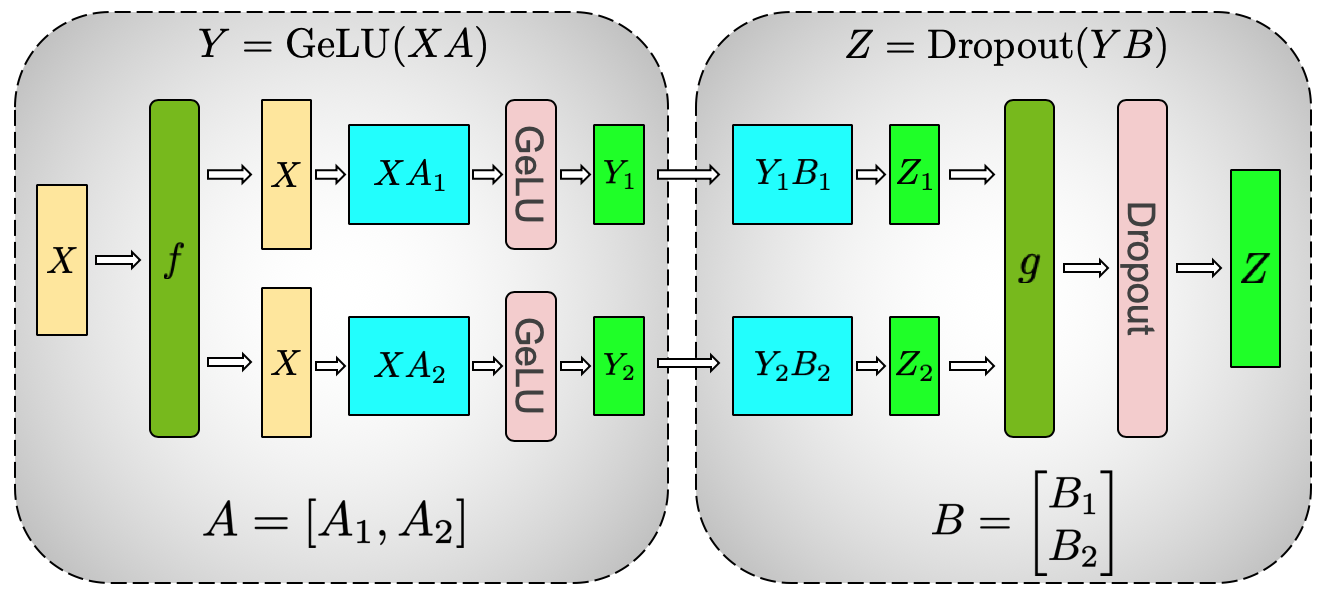
\includegraphics[scale=.3]{figures/mlp_mp_2.png}
 \caption{Tensor parallelism for the \pyinline{MLP} layers. Graphic from
 \cite{shoeybi2020megatronlm}. The $ f/g $ operations are the collective
identity/\pyinline{AllReduce} operations in the forwards pass and the \pyinline{AllReduce}/identity
operations in the backwards pass.}
 \label{fig_mlp_tensor_parallel}
\end{figure}


 \paragraph{Attention} The computations for each the $ H $ individual attention heads, which result
 in the various re-weighted values $ t ^{ h }_{ bsf } $ \eqref{eq_reweighted_values}, can be
 partitioned arbitrarily across workers without incurring any collective communications costs.  Each
 worker then holds some subset of these $ h \in \left \{ 0, \ldots , H-1 \right \} $ activations and
 the final output matrix multiply can be schematically broken up as in \begin{align} &{\rm Concat}
     \left ( \left [ t ^{ 0 }, \ldots , t ^{ H-1 } \right ] \right ) \cdot O \nn &= {\rm Concat}
     \left ( \left [ {\rm Concat}\left ( \left [ t ^{ 0 }, \ldots , t ^{ \frac{ H }{ T }-1 } \right
     ] \right ) \cdot O ^{ (0) }, \ldots ,{\rm Concat}\left ( \left [ t ^{ H-\frac{ H }{ T } },
\ldots , t ^{ H} \right ] \right ) \cdot O ^{ (T-1) } \right ] \right ) \ , \end{align} where matrix
products and concatenation both occur along the hidden dimension. That is, each worker in a group
has $ H/T $ different \pyinline{(B, S, D/H)}-shaped activations $ t ^{ h } $, which can be
concatenated into a \pyinline{(B, S, D/T)}-shaped tensor and multiplied into the
\pyinline{(D/T, D)}-shaped shard of $ O $ whose dimensions correspond to those in the just-concatenated tensor.
Concatenating together each such result from every worker (via an \pyinline{AllReduce}) gives the
desired output. The backwards pass requires similar collective communications to the \pyinline{MLP}
case above.


 \begin{figure}[ht]
     \centering
     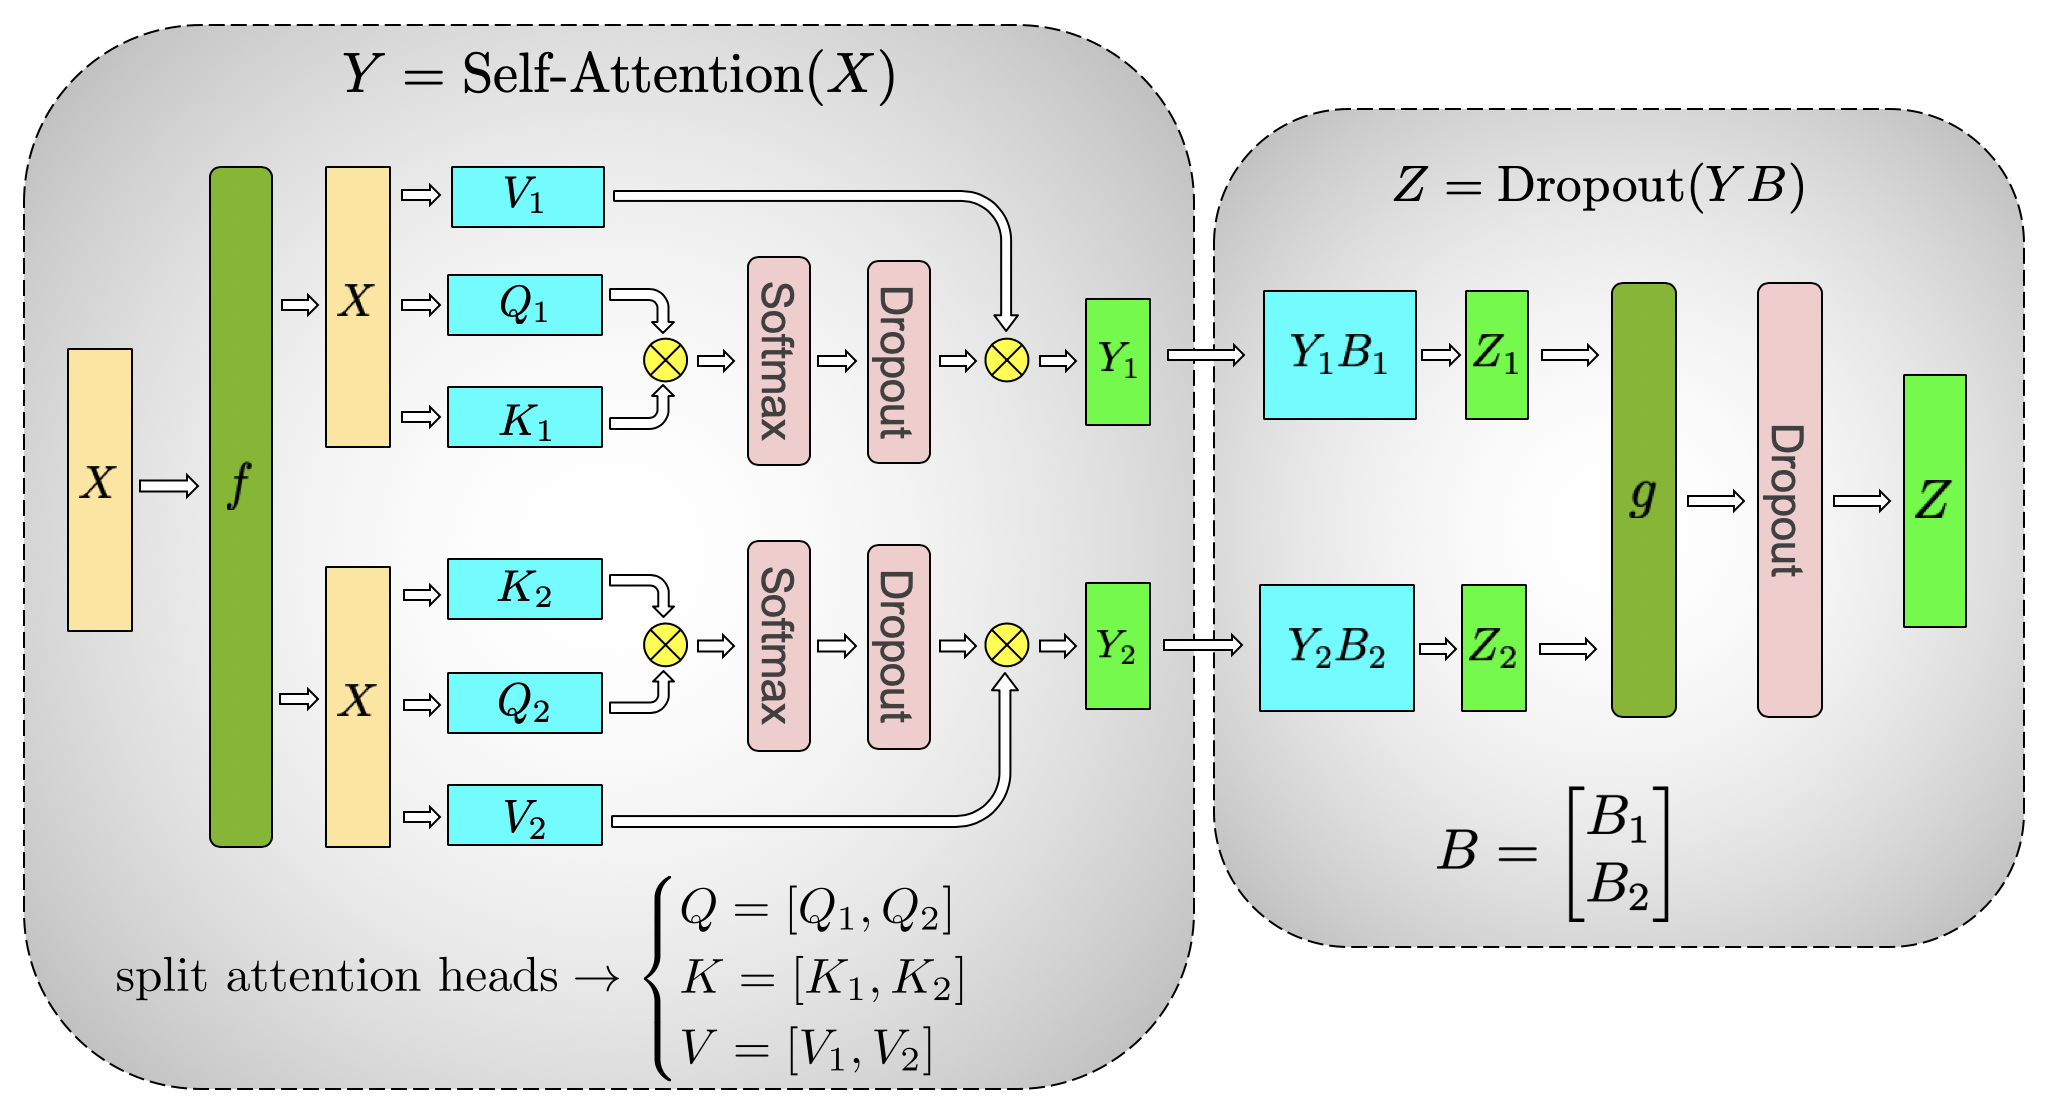
\includegraphics[scale=.3]{figures/attention_mp_2.png}
     \caption{Tensor parallelism for the \pyinline{CausalAttention} layers. Graphic from
     \cite{shoeybi2020megatronlm}. }
     \label{fig_attn_tensor_parallel}
 \end{figure}


 \paragraph{Effects on Memory} The per-worker memory savings come from the sharding of

\subsection{Pipeline Parallelism}


\subsection{Sequence Parallelism}

\subsection{Case Study: Mixed-Precision GPT3 \label{subsec_gpt_mem_study} }
Let's run through the numbers for mixed-precision GPT3 with
\href{https://bmk.sh/2020/05/29/GPT-3-A-Brief-Summary/}{parameters}:
\begin{align}
L &= 96 \ ,
D = 12288 \ ,
H = 96\ , V = 50257\ .
 \label{eq_gpt_num}
\end{align}
We are leaving the sequence-length unspecified, but the block-size (maximum sequence-length) is $
K=2048 $


Start by assuming no parallelism at all. The total non-activation memory is
\begin{align}
  M _{ {\rm non-act}  } ^ \texttt{GPT-3} & \approx 730\ {\rm TiB}
\end{align}
which can be broken down further as
\begin{align}
  M _{ {\rm params}  } ^ \texttt{GPT-3} & \approx 80\ {\rm TiB} \ ,
 M _{ {\rm grads}  } ^ \texttt{GPT-3}  \approx 160\ {\rm TiB}\ ,
  M _{ {\rm optim}  } ^ \texttt{GPT-3}  \approx 490\ {\rm TiB}\ .
\end{align}
The vocabulary only makes up $ \approx .3\% $ of the total number of parameters, so the $ \Ocal
\left( VD \right)  $ term in \eqref{eq_approx_params} is negligible.


The activation memory is
\begin{align}
  M _{ {\rm act}  } ^ \texttt{GPT-3} & \approx 3 \times 10 ^{ -2 }BS\times  \left (  1  + \frac{ S
  }{ 10 ^{ 3 } } \right ) \ {\rm TiB} \ .
\end{align}
Note attention matrices, which are responsible for $ \Ocal \left( S ^{ 2 } \right)  $ term, will
provide the dominant contribution to activation memory in the usual $ S \gtrsim 10 ^{ 3 } $ regime.

In the limit where we process the max block size ($ S=K=2048 $), the ratio of activation to
non-activation memory is
\begin{align}
  \frac{  M _{ {\rm act}  } ^ \texttt{GPT-3}}{ M _{ {\rm non-act}  } ^ \texttt{GPT-3} }\Big| _{
  S=2048 } & \approx  .2 B \ .
\end{align}
So, the activation memory is very significant for such models.



\section{FLOPS}




\part{Inference}







\appendix


\section{Conventions and Notation}\label{app_conventions}


We loosely follow the conventions of \cite{korthikanti2022reducing} and denote the main Transformers
parameters by:
\begin{itemize}
\item $ B $: microbatch size
\item $ K $: the block size (maximum sequence length\footnote{In the absence of methods such as
    ALiBi \cite{ALiBi}  can be used to extend the sequence length at inference time.})
\item $ S $: input sequence length
\item $ V $: vocabulary size
\item $ D $: the hidden dimension size
\item $ L $: number of transformer layers
\item $ H $: number of attention heads
\item $ P $: pipeline parallel size
\item $ T $: tensor parallel size
\item $ E $: expansion factor for MLP layer (usually $ E=4 $)
\end{itemize}
Where it makes sense, we try to use the lower-case versions of these characters to denote the
corresponding indices on various tensors. For instance, an input tensor with the above batch size,
sequence length, and vocabulary size would be written as $ x _{ bsv } $, with $ b \in \left \{ 0,
\ldots, B - 1 \right \} $, $ s \in \left \{ 0, \ldots, S - 1\right \} $, and $  v \in \left \{ 0,
    \ldots, V -1\right \}$ in math notation, or as \mintinline{python}{x[b, s, v]} in code.  Typical
    transformers belong to the regime
\begin{gather}
V \gg D, S \gg L, H \gg P, T \ .  \label{app_eq_transformers_approxs}
\end{gather}


As indicated above,  we use zero-indexing. We also use \pyinline{python} code
throughout\footnote{Written in a style conducive to latex, e.g. no type-hints and pegagogy
prioritized.}  and
write all ML code using standard \pyinline{torch} syntax. To avoid needing to come up with new
symbols in math expressions we will often use expressions like $ x \leftarrow f(x) $ to refer to performing
a computation on some argument ($ x $) and assigning the result right back to the variable $ x $
again.

Physicists often joke (half-seriously) that Einstein's greatest contribution to physics was his
summation notation in which index-sums are implied by the presence of repeated indices and summation
symbols are entirely omitted. For instance, the dot product between two vectors would be written as
\begin{align}
    \vec{x} \cdot \vec{y} &= \sum _{ i } x _{ i } y _{ i } \equiv x _{ i } y _{  i }
    \label{app_eq_einstein_sum}
\end{align}
We use similar notation which is further adapted to the common element-wise deep-learning
operations.  The general rule is that if a repeated index appears on one side of an equation, but
not the other, then a sum is implied, but if the same index appears on both sides, then it's an
element-wise operation. The Hadamard-product between two matrices $ A $ and $ B $ is just
\begin{align}
  C _{ ij } &= A _{ ij } B _{ ij }\ .
\end{align}
Einstein notation also has implementations available for \pyinline{torch}:
\href{https://rockt.github.io/2018/04/30/einsum}{see this blog post on \pyinline{einsum}} or the
\href{https://einops.rocks/1-einops-basics/}{\pyinline{einops}} package.

 We also put explicit indices on operators such as Softmax to help clarify the relevant
 dimension, e.g. we would write the softmax operation over the $ b $-index of some batched
 tensor $ x _{ bvd\ldots } $ as
 \begin{align}
     s _{ bvd\ldots } &= \frac{ e^{ x _{ bv d\ldots}  } }{ \sum _{ v = 0 } ^{  v= V-1 } e^{ x _{
     bvd\ldots } } } \equiv
     \Sm _{ v } \ x _{ bvd\ldots }
     \ , \label{app_eq_einstein_softmax}
 \end{align}
 indicating that the sum over the singled-out $ v $-index is gives unity.

\section{Collective Communications \label{app_collective_communications} }

A quick refresher on common distributed
\href{https://docs.nvidia.com/deeplearning/nccl/user-guide/docs/usage/collectives.html}{communication
primitives}.  Consider $ N $ workers with tensor data $ x ^{ (n) }  $ of some arbitrary shape
\pyinline{x.shape}, where $ n $ labels the worker and any indices on the data are suppressed. The $
n=0 $ worker is arbitrarily denoted the \textit{chief}.  Then, the primitive operations are:
\begin{itemize}
    \item \pyinline{Broadcast}: all workers receive  the chief's data, $ x ^{ (0) }  $.
    \item \pyinline{Gather}: all workers communicate their data $ x _{ n } $ to the chief, e.g. in a
        concatenated array $ [x ^{ 0 }, x ^{ 1 }, \ldots , x ^{ N-1 }] $.
    \item \pyinline{Reduce}: data is \pyinline{Gather}-ed to the chief, which then performs some
        operation (\pyinline{sum}, \pyinline{max}, \pyinline{concatenate}, etc.) producing a new tensor $
        x' $ on the chief worker.
    \item \pyinline{AllGather}: \pyinline{Gather} followed by \pyinline{Broadcast}, such that all
        data $ x ^{ (n) } $ is communicated to all workers.
    \item \pyinline{AllReduce}: generalization of \pyinline{Reduce} where all
        workers receive the same tensor $ x' $ produced by operating on the $ x ^{ (n) } $.
        Equivalent to a \pyinline{Reduce} followed by \pyinline{Broadcast}, or a
        \pyinline{ReduceScatter} followed by a \pyinline{AllGather} (the more efficient choice).
    \item \pyinline{ReduceScatter}: a reducing operation is applied to the $ x ^{ (n) } $ to produce
        a $ x' $ of the same shape, but each worker only receives a slice $ 1/N $ of the result.
\end{itemize}

 \section{TODO}


 \begin{itemize}
 \item Tokenizers
 \item Generation
 \item Activations
 \item Flash attention
 \item BERT family
 \item Residual stream
 \item Scaling laws
 \end{itemize}

\bibliographystyle{latex_goon/utphys}
\bibliography{bibliography}
\end{document}




